\documentclass[../../main.tex]{subfiles}
\usepackage{pgfplots}
\pgfplotsset{compat=1.17}
\begin{document}
\chapter{Rigging and Layers}
\label{ch:rigging_layers}

In computer graphics, rigging involves setting up a skeletal structure (also known as an armature) that drives the mesh of a character, allowing it to move and deform in a realistic manner. Rigging is a critical component of character animation, as it determines how the character responds to movement and how it deforms during animation. In the context of sign language avatars, rigging plays a crucial role in capturing the complex articulations and expressions of sign language gestures.

The layered approach to rigging, which this chapter explores in depth, offers a sophisticated method for managing these complexities. By dividing the rigging process into several distinct layers—each responsible for a different aspect of the avatar’s movement and deformation—we can achieve a higher level of control and flexibility. This approach not only facilitates the creation of more natural and expressive animations but also makes the system scalable and adaptable to a wide range of linguistic contexts.

In this chapter, section \ref{ch:rigging_layers:proc_rig_signing_avatars} introduces a procedural rigging system for signing avatars, which automates the rigging process and enables the generation of complex sign language gestures. Section \ref{ch:rigging_layers:results} presents the results of the implementation, and section \ref{ch:rigging_layers:evaluation} evaluates the performance, accuracy, and quality of the animation. Finally, section \ref{ch:rigging_layers:conclusion} concludes the chapter and discusses future work.

\section{Procedural Rigging for Signing Avatars}
\label{ch:rigging_layers:proc_rig_signing_avatars}

Rigs have been used in computer animation for decades to control the movement and deformation of characters. Traditional rigging systems typically consist of a hierarchical structure of bones, controllers, and constraints that define how the character’s mesh deforms in response to movement.

A signing avatar differs significantly from the traditional systems. For starter, no sign language uses the lower body in its articulation. This means that the rigging system for a signing avatar can be simplified to focus on the upper body as shown in figure \ref{ref:upper_body_avatar}. 

\begin{figure}[h]
    \centering
    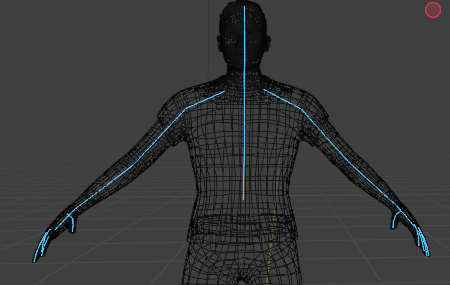
\includegraphics[width=0.5\textwidth]{chapters/rigging_layers/images/upper_body_avatar.png}
    \caption{An example of an upper body avatar rig}
    \label{ref:upper_body_avatar}
\end{figure}

However for procedurally animating a signing avatar, the complexity of sign language gestures and expressions poses unique challenges and necessitates a more sophisticated rigging system.

\subsection{AZee Blender interface}
\label{ch:rigging_layers:proc_rig_signing_avatars:azee_blender_interface}

The previous low level synthesizor for AZee \cite{fabrizio} was based on an armature in blender. These bones and sites were mapped to a \emph{SkelSpec} structure. Similarly, AZee's abstract posture was mapped to the \emph{SkelSpec} structure as well. The \emph{SkelSpec} structure thus formed as an intermediate bridge between an Animated AZee Score and the armature \ref{fig:old_interface}. 

\begin{figure}
    \centering
    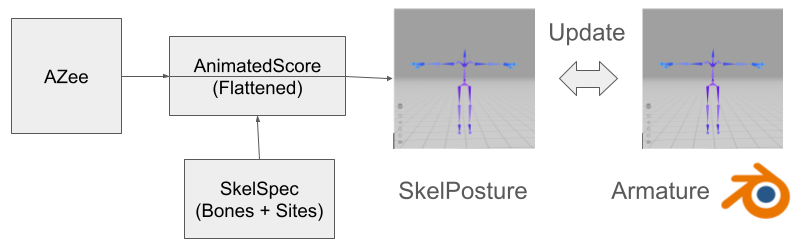
\includegraphics[width=0.5\textwidth]{chapters/rigging_layers/images/old_interface.png}
    \caption{The old interface of the low level synthesizor for AZee}
    \label{fig:old_interface}
\end{figure}

One of the first contributions of this work was to create a new interface for the low level synthesizor for AZee. This new interface didn't have a \emph{SkelSpec} \ref{fig:new_interface} and interacted directly with the blender armature. 

\begin{figure}
    \centering
    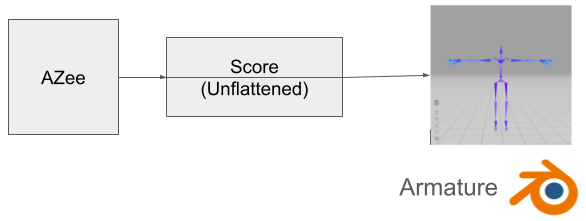
\includegraphics[width=0.5\textwidth]{chapters/rigging_layers/images/new_interface.png}
    \caption{The new interface of the low level synthesizor for AZee}
    \label{fig:new_interface}
\end{figure}

\subsection{Automatic site generation}
\label{ch:rigging_layers:proc_rig_signing_avatars:auto_site_generation}

The AZee low-level language consists of 332 sites (appendix \ref{appendix:sites}) which the user to manually create sites in blender. This was a tedious time consuming process process and could lead to errors \ref{fig:prev_sites}.

\begin{figure}
    \centering
    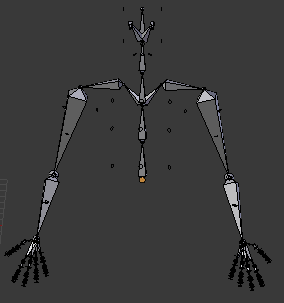
\includegraphics[width=0.5\textwidth]{chapters/rigging_layers/images/prev_sites.png}
    \caption{Manually created sites in the previous low level synthesizor for AZee}
    \label{fig:prev_sites}
\end{figure}

This site generation process could be partially automated if we have the knowledge of the bone structure. Algorithm was used to generate sites based on bone location and avatar mesh using simple raycasting \ref{alg:site_generation_with_raycasting}.

\begin{algorithm}
    \label{alg:site_generation_with_raycasting}
    \caption{Raycasting Algorithm for Automatic Site Generation}
    \begin{algorithmic}
        \State \textbf{Input:} A 3D model with bones
        \State \textbf{Output:} Generated and positioned sites on the model

        \State $sites \gets$ an empty list to store generated site locations

        \State \text{Remove existing sites from the model}

        \State $armature \gets$ find the armature associated with the 3D model

        \For{each $bone$ in $armature$}
            \State $start\_point \gets$ determine a starting point based on the bone's position
            \State $direction \gets$ calculate the direction vector based on the bone's orientation
            
            \State $hit\_success, hit\_location \gets$ perform raycasting from $start\_point$ in $direction$
            \If{$hit\_success$}
                \State $site\_location \gets hit\_location$
            \Else
                \State $site\_location \gets$ fallback location based on predefined logic
            \EndIf

            \State add $site\_location$ to $sites$ list
            
            \State \text{Apply any additional constraints or relationships between the site and the bone}
        \EndFor

        \For{each $finger$ in the model's fingers}
            \For{each $segment$ in $finger$}
                \State repeat the raycasting procedure to determine and store $site\_locations$ for each segment
            \EndFor
        \EndFor

        \State finalize and store the $sites$ list for further processing or rendering
    \end{algorithmic}
\end{algorithm}

The sites an be visualized on the avatar in figure \ref{fig:sites_bazeel_combined}.

\begin{figure}[h]
    \centering
    \begin{subfigure}[b]{0.3\textwidth}
        \centering
        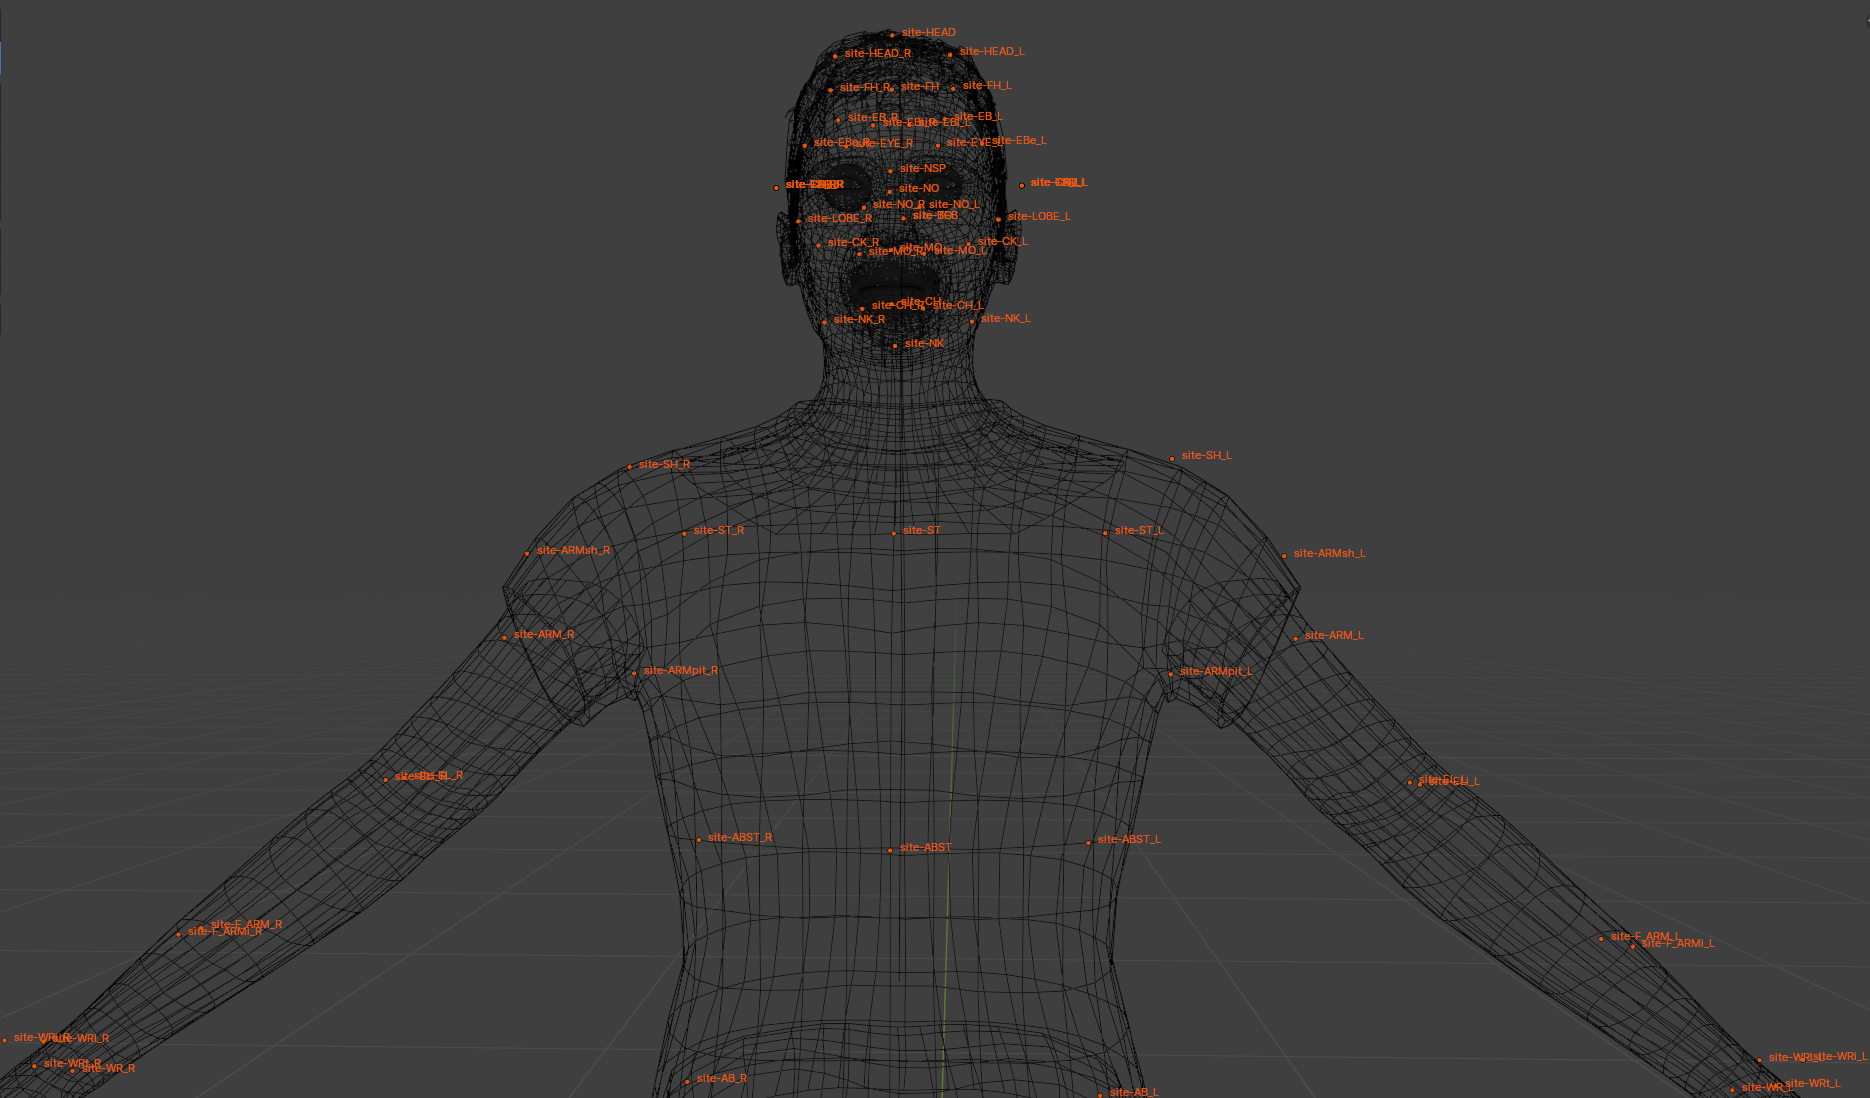
\includegraphics[width=\textwidth]{chapters/rigging_layers/images/sites_body_front.png}
        \caption{Front View of Body Sites}
        \label{fig:sites_body_front}
    \end{subfigure}
    \hfill
    \begin{subfigure}[b]{0.3\textwidth}
        \centering
        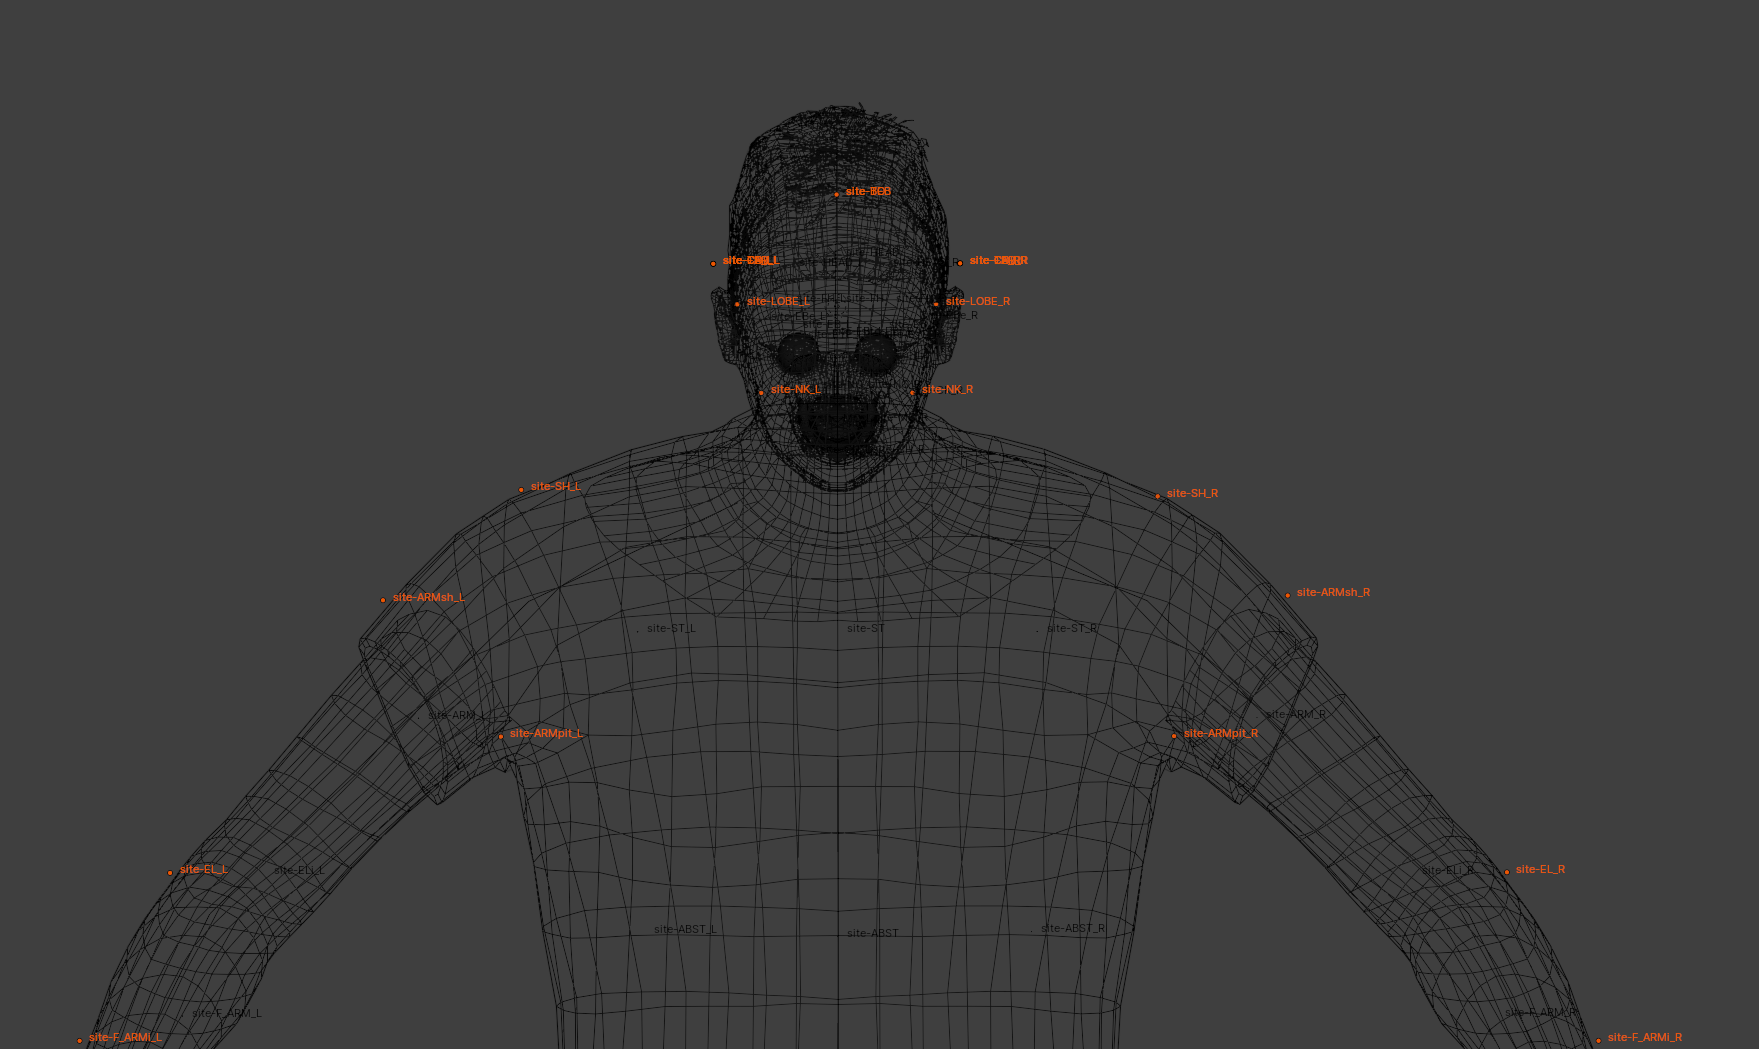
\includegraphics[width=\textwidth]{chapters/rigging_layers/images/sites_body_back.png}
        \caption{Back View of Body Sites}
        \label{fig:sites_body_back}
    \end{subfigure}
    \hfill
    \begin{subfigure}[b]{0.3\textwidth}
        \centering
        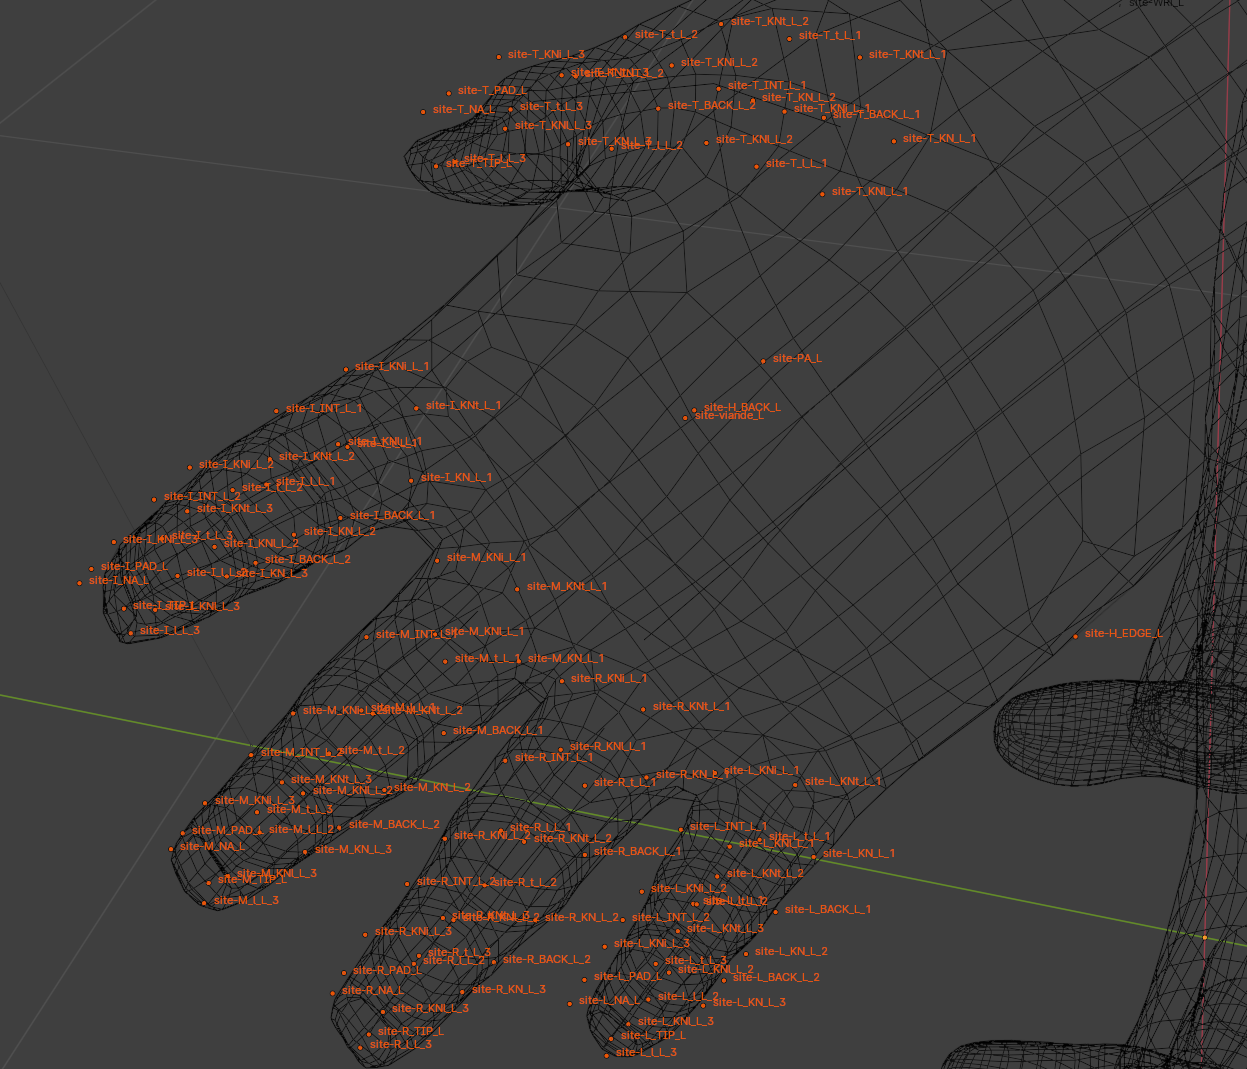
\includegraphics[width=\textwidth]{chapters/rigging_layers/images/sites_hand.png}
        \caption{Hand Sites}
        \label{fig:sites_hand}
    \end{subfigure}
    \caption{AZee sites on the BAZeel avatar: Front and Back Body Views, and Hand Sites}
    \label{fig:sites_bazeel_combined}
\end{figure}

\subsection{Automatic rigging}
\label{ch:rigging_layers:proc_rig_signing_avatars:auto_rig}

The previous custom rig contained 57 bones \ref{appendix:old_bone_list}. These bones were initially structured to accommodate the unique skeletal system requirements of the AZee framework, which utilizes a "rotation first" paradigm. However, since Blender operates on a "translation first" paradigm, a conversion process was necessary. This conversion involved splitting each AZee bone into two corresponding Blender bones: one for translation and one for rotation, with the rotation bone named by appending a ".rot" suffix to the original bone name (figure \ref{fig:old_bone_structure}). Additionally, sites were modeled in a dual fashion, where both bones and empty objects were created to manage site positioning and visualization.

\begin{figure}
    \centering
    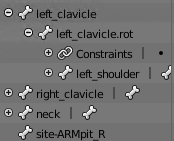
\includegraphics[width=0.5\textwidth]{chapters/rigging_layers/images/old_bone_structure.png}
    \caption{Duplicate bones for rotation and translation}
    \label{fig:old_bone_structure}
\end{figure}

This old system however, can be improved using multiple avatar layers. To do this we need 3 separate layers,

\subsection{Deformation Bone Layer}
\label{ch:rigging_layers:proc_rig_signing_avatars:deform_bone_layer}

The deformation bone layer(figure \ref{ref:deform_layer}) is the foundation of the avatar's rig. It includes the bones that directly influence the mesh of the character, controlling how the skin deforms in response to movement. This layer is responsible for the overall shape and posture of the avatar, ensuring that the character's movements are smooth and realistic.

In this layer, the bones are typically organized into a hierarchy, with the root bone controlling the overall position and orientation of the avatar, and child bones controlling specific parts of the body, such as the limbs, spine, and head. Weight painting is used to determine how much influence each bone has over the surrounding mesh, allowing for precise control over how the character's skin deforms.

\begin{figure}
    \centering
    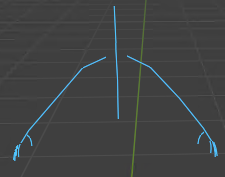
\includegraphics[width=0.5\textwidth]{chapters/rigging_layers/images/deform_layer.png}
    \caption{Deformation bone layer}
    \label{fig:deform_layer}
\end{figure}

\subsection{Inverse Kinematics Layer}
\label{ch:rigging_layers:proc_rig_signing_avatars:ik_layer}

The inverse kinematics (IK) layer (figure ref:ik_layer) is responsible for positioning the avatar's limbs and spine by solving for the joint angles required to achieve a desired end-effector position.

A separate IK layers ensures that the FK configuration is not lost during constraint evaluation. If the posture is in IK mode i.e. is solving for a placement, the deform layers copy the orientations resolved by the IK layer.

\begin{figure}
    \centering
    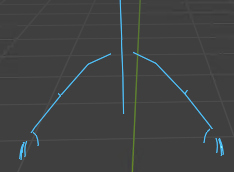
\includegraphics[width=0.5\textwidth]{chapters/rigging_layers/images/ik_layer.png}
    \caption{IK bone layer}
    \label{fig:ik_layer}
\end{figure}

\subsection{Forward Kinematics Layer}
\label{ch:rigging_layers:proc_rig_signing_avatars:fk_layer}

The forward kinematics (FK) layer (figure \ref{fig:fk_layer}) controls the rotation of bones in a hierarchical manner, where the rotation of a parent bone affects all its children. This layer is used for broader, more deliberate movements, such as head tilts, body leans, or full-body rotations, which are important for conveying non-manual signals in sign language.

FK provides animators with a high degree of control over each individual bone in the rig, allowing for precise adjustments to the character's pose. Unlike IK, where the position of the end-effector is specified, FK requires the animator to manually rotate each bone in the chain, starting from the root and working down to the extremities. This can be more time-consuming but offers greater flexibility in achieving complex poses.

\begin{figure}
    \centering
    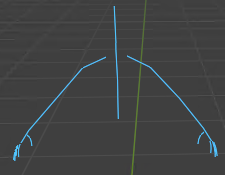
\includegraphics[width=0.5\textwidth]{chapters/rigging_layers/images/fk_layer.png}
    \caption{FK bone layer}
    \label{fig:fk_layer}
\end{figure}

\subsection{Constraint Based Posture Optimization}
\label{ch:rigging_layers:proc_rig_signing_avatars:cb_posegen}

The previous low level synthesizor for AZee \cite{fabrizio} used a constraint based optimization algorithm to generate the armature pose for a frame. This algorithm \ref{alg:old_constraint_optimization} collects all posture constaints given by the AZee Animated Score for every frame and solves for the posture by optimizing this constraints using distance functions. 

\begin{algorithm}
    \caption{Constraint-Based Optimization for Posture Synthesis}
    \label{alg:trimmed_constraint_based_optimization}
    \begin{algorithmic}[1]
    \Require $\text{PostureConstraints} \ \mathit{posture\_constraint}$, $\text{Object} \ \mathit{armature\_object}$
    \Ensure Armature object is posed according to the constraints
    
    \State \textbf{Initialize:} $i \gets 0$
    \State $distance\_threshold \gets \mathit{bpy.context.scene.azee\_ik\_site\_distance\_threshold}$
    \State $angle\_threshold \gets \mathit{bpy.context.scene.azee\_ik\_bone\_rot\_angle\_threshold \times \pi / 180}$
    \State $max\_iterations \gets \mathit{bpy.context.scene.azee\_ik\_max\_iterations}$
    
    \While{$i < max\_iterations$}
        \State \textbf{Apply Constraints:} \textsc{ApplyPositionConstraint}($\mathit{posture\_constraint}$), \textsc{ApplyOrientConstraints}($\mathit{posture\_constraint}$)
        \State \textbf{Compute Offsets:} $place\_distance, orient\_angles \gets \textsc{ComputeDistance}(\mathit{posture\_constraint})$
        \If {$\mathit{place\_distance} < \mathit{distance\_threshold}$ \textbf{and} $\max(\mathit{orient\_angles}) < \mathit{angle\_threshold}$}
            \State \textbf{Break:} \textbf{end while}
        \EndIf
        \State $i \gets i + 1$
    \EndWhile
    
    \Procedure{ApplyPositionConstraint}{$\mathit{posture\_constraint}$}
        \If {$\mathit{posture\_constraint.place\_constraint} \neq \text{None}$}
            \State \textbf{Apply IK:} \textsc{ApplyIKConstraint}($\mathit{posture\_constraint.place\_constraint.site\_pose\_bone}$, 
            \textsc{CreateTemporaryTarget}($\mathit{posture\_constraint.place\_constraint.target\_vect}$), \textit{position})
        \EndIf
    \EndProcedure
    
    \Procedure{ApplyOrientConstraints}{$\mathit{posture\_constraint}$}
        \ForAll {$orient\_constraint \in \mathit{posture\_constraint.orient\_constraints}$}
            \State \textbf{Apply IK:} \textsc{ApplyIKConstraint}($orient\_constraint.pose\_bone$, 
            \textsc{CreateTemporaryTarget}($orient\_constraint.get\_target\_quaternion()$), \textit{rotation}, 
            $orient\_constraint.get\_axis\_relaxation\_mask()$)
        \EndFor
    \EndProcedure
    
    \Procedure{ComputeDistance}{$\mathit{posture\_constraint}$}
        \State \Return \textsc{ComputeDistanceFromOffset}(\textsc{ComputePlaceOffset}($\mathit{posture\_constraint}$)), 
        \textsc{ComputeAnglesFromOffsets}(\textsc{ComputeOrientOffsets}($\mathit{posture\_constraint}$))
    \EndProcedure
    \end{algorithmic}
\end{algorithm}

The approach handles only placements and orientations and uses a flattened animated AZee Score. This was improved \ref{alg:new_constraint_optimization} by generating from the multi-track synced score itself(more discussed in chapter \ref{ch:multi-track}) with support for other constraints such as \emph{morph}, \emph{lookat} and \emph{trill}.

\begin{algorithm}
    \caption{Constraint-Based Optimization for Posture Synthesis}
    \label{alg:trimmed_multi_track_optimization}
    \begin{algorithmic}[1]
        \Require $\text{PostureConstraints} \ \mathit{posture\_constraint\_DAG}$, $\text{Object} \ \mathit{armature\_object}$, $\text{FrameRange} \ \mathit{frames}$
        \Ensure Armature object is posed according to the constraints
        
        \State \textbf{Initialize:} $i \gets 0$
        \State $distance\_threshold \gets \mathit{bpy.context.scene.azee\_ik\_site\_distance\_threshold}$, $angle\_threshold \gets \mathit{bpy.context.scene.azee\_ik\_bone\_rot\_angle\_threshold \times \pi / 180}$
        \State $max\_iterations \gets \mathit{bpy.context.scene.azee\_ik\_max\_iterations}$
        \State $\mathit{sorted\_constraints} \gets \mathit{posture\_constraint\_DAG.topological\_sort()}$
        \State $frames\_to\_keyframe \gets \textsc{DetermineFramesToKeyframe}(\mathit{frames}, \mathit{dynamic\_points})$
        
        \While{$i < max\_iterations$}
            \ForAll {$f \in \mathit{frames\_to\_keyframe}$}
                \State $\mathit{cumulative\_loss} \gets 0.0$
                \ForAll {$constraint \in \mathit{sorted\_constraints}$}
                    \State \textbf{Apply Constraint:} \textsc{ApplyConstraint}($constraint$, $f$)
                    \State $\mathit{cumulative\_loss} \gets cumulative\_loss + \mathit{constraint.get\_loss(f)}$
                \EndFor
                \If {$cumulative\_loss < \mathit{bpy.context.scene.azee\_animator\_threshold}$}
                    \State \textbf{Break:} \textbf{end while}
                \EndIf
                \State \textbf{Insert Keyframe:} \textsc{InsertKeyframe}($f$)
            \EndFor
            \State $i \gets i + 1$
        \EndWhile
        
        \Procedure{ApplyConstraint}{$constraint, frame$}
            \If {$constraint$ \textbf{is} PlacementConstraint}
                \State \textsc{PlaceSite}($constraint.site$, \textsc{EvaluatePlacementTarget}($constraint$, $frame$))
            \ElsIf {$constraint$ \textbf{is} OrientationConstraint}
                \State \textsc{RotateBone}($constraint.bone$, \textsc{EvaluateOrientation}($constraint$, $frame$))
            \ElsIf {$constraint$ \textbf{is} MorphConstraint}
                \State \textsc{ApplyMorph}($constraint$, $frame$)
            \ElsIf {$constraint$ \textbf{is} LookAtConstraint}
                \State \textsc{RotateEyesToTarget}($constraint.eyes$, \textsc{EvaluateLookAtPoint}($constraint$, $frame$))
            \ElsIf {$constraint$ \textbf{is} TrillConstraint}
                \State \textsc{ApplyTrill}($constraint$, $frame$)
            \ElsIf {$constraint$ \textbf{is} TranspathConstraint}
                \State \textsc{FollowPath}($constraint.site$, \textsc{DeterminePath}($constraint$, $frame$))
            \Else
                \State \textsc{HandleError}()
            \EndIf
        \EndProcedure
        
        \Procedure{DetermineFramesToKeyframe}{$frames, dynamic\_points$}
            \State \Return $\textsc{IdentifyKeyFrames}(\mathit{frames}) \cup \textsc{DynamicFrameRanges}(dynamic\_points)$
        \EndProcedure
        
        \Procedure{InsertKeyframe}{$frame$}
            \ForAll {$fcurve \in \mathit{armature\_object.animation\_data.action.fcurves}$}
                \State \textsc{KeyframeInsert}($fcurve$, $frame$)
            \EndFor
        \EndProcedure
    \end{algorithmic}
\end{algorithm}

todo joint limits

\subsection{Morphs Constraints}
\label{ch:rigging_layers:proc_rig_signing_avatars:morph_constraints}

todo dynamic morphs 

The word "morph" comes from the Greek word "morphē" (μορφή), which means "form" or "shape." In modern usage, "morph" is often used as a shorthand for "morphing". In the field of computer graphics and animation, morphs are predefined shape keys that modify the mesh of the avatar independently of the skeletal structure, allowing for the detailed control of specific aspects of the avatar's appearance that cannot be easily achieved through bone manipulation alone. This includes subtle facial expressions, muscle bulges, and other nuanced gestures that are critical for conveying meaning in sign language.

AZee sees morphs as any change in the configuration of the avatar, which can be specified by the linguist in 1 dimension. For instance, closing of hands(a change in skeleton configuration) or raising the eyebrows(a change in the 3D mesh). The syntax of a morph constraint is as follows:

\[
\texttt{morph } \text{\emph{'morph\_id'}} \ \texttt{weight[0, 1]}
\]

\subsubsection{Skeletal Morphs}
\label{ch:rigging_layers:proc_rig_signing_avatars:morph_constraints:skel_morphs}

Skeletal morphs are a specific type of morph that directly manipulates the skeletal structure of an avatar to produce a desired pose or motion. Unlike traditional bone-based manipulations that rely solely on inverse or forward kinematics, skeletal morphs allow for more nuanced and localized control over specific joints or groups of joints. This is particularly useful for complex hand gestures or other detailed movements that are difficult to achieve with bone rotations alone.

In AZee, skeletal morphs are treated as constraints that define a forward kinematic change in the avatar's skeletal configuration. These morphs can influence various aspects of the skeleton, such as:

\begin{itemize}
    \item \textbf{Flexion and Extension:} This refers to the bending (flexion) or straightening (extension) of a joint, such as the fingers or wrists. Flexion reduces the angle between bones, while extension increases it.
    \item \textbf{Adduction and Abduction:} Adduction involves moving a limb closer to the body's midline, whereas abduction moves it away. These movements are crucial for natural arm and hand gestures.
    \item \textbf{Hyperextension:} This is an extension of a joint beyond its normal range of motion, often used for expressive gestures that require exaggerated poses.
\end{itemize}

Figure \ref{fig:skeletal_morphs} shows a table of skeletal morphs and their corresponding effects on the avatar's skeleton.

todo
\begin{figure}
    \centering
    \begin{tabular}{|c|c|}
        \hline
        \textbf{Morph ID} & \textbf{Effect} \\
        \hline
        \texttt{hand\_close} & Closes the hand into a fist \\
        \texttt{hand\_open} & Opens the hand from a fist \\
        \texttt{wrist\_flex} & Bends the wrist downwards \\
        \texttt{wrist\_extend} & Straightens the wrist \\
        \texttt{elbow\_flex} & Bends the elbow \\
        \texttt{elbow\_extend} & Straightens the elbow \\
        \texttt{shoulder\_adduct} & Moves the shoulder towards the body's midline \\
        \texttt{shoulder\_abduct} & Moves the shoulder away from the body's midline \\
        \texttt{shoulder\_hyperextend} & Hyperextends the shoulder \\
        \hline
    \end{tabular}
    \caption{Table of skeletal morphs and their effects}
    \label{fig:skeletal_morphs}
\end{figure}

\subsubsection{Facial Morphs}
\label{ch:rigging_layers:proc_rig_signing_avatars:morph_constraints:facial_morphs}

Facial morphs in the AZee framework provide a means to represent the complex and nuanced expressions essential for conveying emotions and grammatical cues in sign languages. These morphs are crucial for enhancing the realism and expressiveness of signing avatars, allowing them to replicate the subtle facial movements that are integral to effective communication in sign language (figure \ref{fig:facial_example}).

\begin{figure}
    \centering
    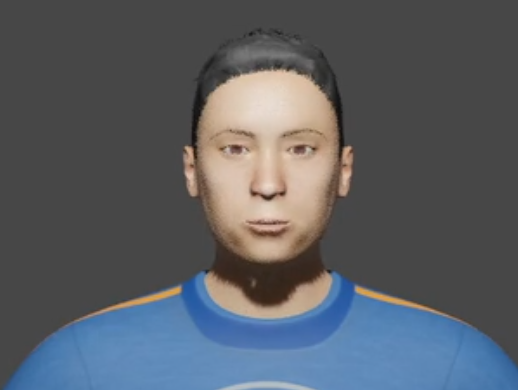
\includegraphics[width=0.5\textwidth]{chapters/rigging_layers/images/facial_example.png}
    \caption{Facial morph for ..todo}
    \label{fig:facial_example}
\end{figure}

Facial Morph targets are typically generated by sculpting the avatar's mesh into various shapes that correspond to different expressions or gestures. These sculpted shapes are then saved as "keys," which can be blended together during animation to produce the desired expression. This process allows for a high degree of flexibility in animation, as different keys can be combined in real-time to create a wide range of expressions. While this section offers a brief overview, the detailed modeling, implementation, and challenges associated with facial morphs are discussed extensively in Chapter \ref{ch:facial_expressions}.

\subsubsection{Integration with other layers}
\label{ch:rigging_layers:proc_rig_signing_avatars:morph_constraints:intergation}

The morph constraints are integrated along with the other constraints in the posture optimization algorithm \ref{alg:posture_morph_integrate}. The skeletal morphs act on the FK layer while the facial morphs act on the mesh directly.

todo
\begin{algorithm}
    \caption{Posture Generation with Constraints}
    \label{alg:posture_morph_integrate}
    \begin{algorithmic}[1]    
    \Procedure{GeneratePosture}{$Blocks$}
        \For{each $Block$ in $Blocks$}
            \State $Constraints \gets \text{TopologicalSort}(\text{CreateDAG}(Block))$
            \For{each $Frame$ from $Block.Start$ to $Block.End$}
                \For{$Epoch \gets 1$ to $MaxEpochs$}
                    \State $Loss \gets 0$
                    \For{each $C$ in $Constraints$}
                        \State \text{Apply}($C$, $Frame$)
                        \State $Loss \gets Loss + \text{ComputeLoss}(C, Frame)$
                    \EndFor
                    \If{$Loss < Threshold$} \textbf{break} \EndIf
                \EndFor
                \State \text{InsertKeyframe}(Frame)
            \EndFor
        \EndFor
    \EndProcedure
    
    \Procedure{Apply}{$C$, $Frame$}
        \If{$C$ is $MorphConstraint$} \State \text{ApplyMorph}($C$, $Frame$)
        \ElsIf{$C$ is $PlacementConstraint$} \State \text{ApplyPlacement}($C$, $Frame$)
        \ElsIf{$C$ is $OrientationConstraint$} \State \text{ApplyOrientation}($C$, $Frame$)
        \EndIf
    \EndProcedure
    
    \end{algorithmic}
\end{algorithm}

todo
\begin{algorithm}
    \caption{Calculate MorphConstraint Loss in Terms of FK}
    \begin{algorithmic}[1]
        \label{alg:morph_constraint_loss}
    \Procedure{ComputeMorphFKLoss}{$\mathbf{p}_{\text{current}}$, $\mathbf{p}_{\text{target}}$, $\mathbf{q}_{\text{current}}$, $\mathbf{q}_{\text{target}}$}
        \State $\text{PositionLoss} \gets \|\mathbf{p}_{\text{current}} - \mathbf{p}_{\text{target}}\|$
        \State $\text{RotationDiff} \gets \mathbf{q}_{\text{current}} \cdot \mathbf{q}_{\text{target}}$
        \State $\text{RotationLoss} \gets 1 - |\text{RotationDiff}|$
        \State $\text{TotalLoss} \gets \lambda_p \times \text{PositionLoss} + \lambda_r \times \text{RotationLoss}$
        \State \Return $\text{TotalLoss}$
    \EndProcedure
    
    \Procedure{ApplyMorphConstraint}{$\text{MorphConstraint}$, $\text{Frame}$}
        \State $\mathbf{p}_{\text{current}}, \mathbf{q}_{\text{current}} \gets \text{ApplyMorph}(\text{MorphConstraint}, \text{Frame})$
        \State $\mathbf{p}_{\text{target}}, \mathbf{q}_{\text{target}} \gets \text{GetTargetState}(\text{Frame})$
        \State $\text{Loss} \gets \text{ComputeMorphFKLoss}(\mathbf{p}_{\text{current}}, \mathbf{p}_{\text{target}}, \mathbf{q}_{\text{current}}, \mathbf{q}_{\text{target}})$
        \State \Return $\text{Loss}$
    \EndProcedure
    
    \end{algorithmic}
\end{algorithm}

\section{Results and Implementation}
\label{ch:rigging_layers:results}

The layered rigging system has been implemented and tested on the BAZeel avatar in blender (figure \ref{fig:layers_example}).

\begin{figure}
    \centering
    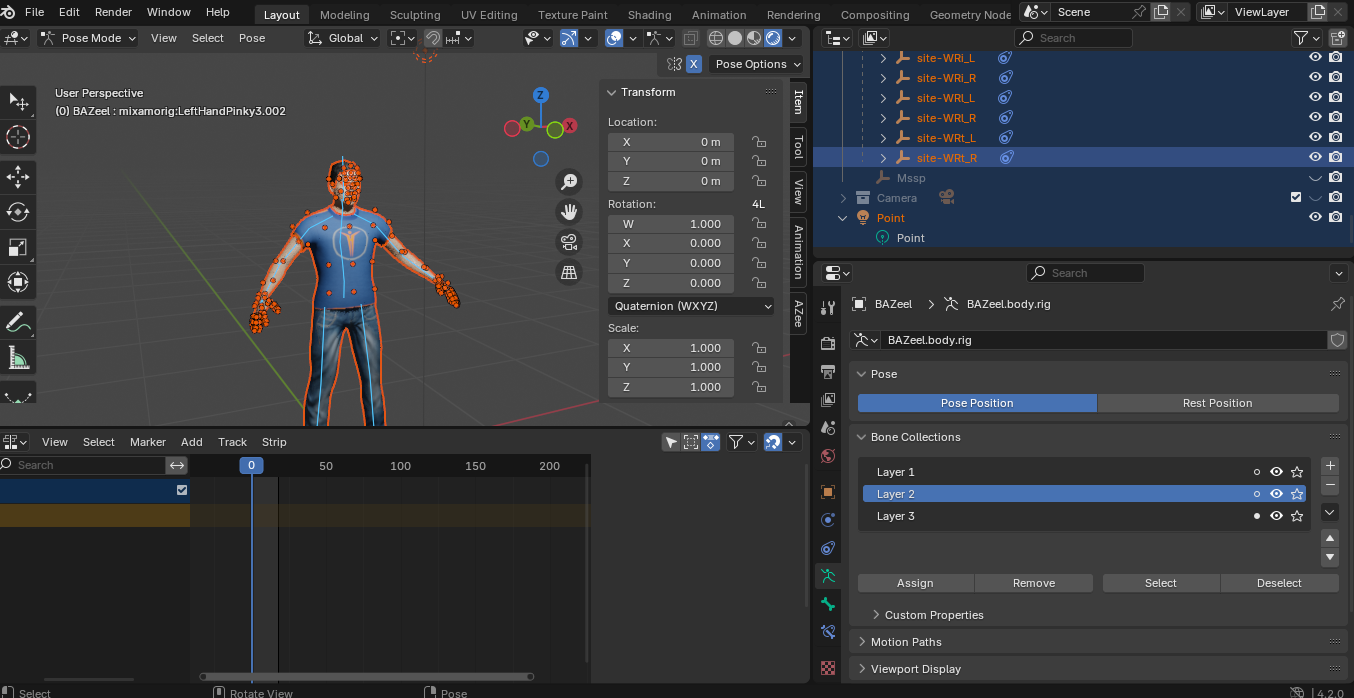
\includegraphics[width=0.5\textwidth]{chapters/rigging_layers/images/layers_example.png}
    \caption{Example of the layered rigging system on the BAZeel avatar}
    \label{fig:layers_example}
\end{figure}

\section{Evaluation}
\label{ch:rigging_layers:evaluation}

\subsection{Performance}
\label{ch:rigging_layers:evaluation:performance}

The animation time compared to the previous synthesizor are shown in table \ref{tab:faster_executions}.

todo
\begin{table}
    \centering
    \begin{tabular}{|c|c|}
        \hline
        \textbf{Interface} & \textbf{Execution time (s)} \\
        \hline
        Old & 0.5 \\
        New & 0.2 \\
        \hline
    \end{tabular}
    \caption{Comparison of execution times between the old and new interfaces}
    \label{tab:faster_executions}
\end{table}

We observe that this synthesis is significantly faster because of direct integration with blender's armature. The automatic site generation and rigging also reduce the time taken to set up the avatar for animation.

\subsection{Accuracy of the Animation}
\label{ch:rigging_layers:evaluation:accuracy}

Frechet gesture distance..todo

against old synthesizor

against state of the art and sgnify

against rosetta mocap

against paula

frobenius distance

\subsection{Quality of Animation}
\label{ch:rigging_layers:evaluation:quality}

As observed, the generated animations are robotic in nature and lack the fluidity and expressiveness of natural sign language gestures. However, everything which can be annotated using the AZee low level, can be synthesized using this technique. This provides us with a good starting block to animate sign language. Moreover, with the procedural rigging system, we can us this same system with other avatars as well.

\section{Conclusion}
\label{ch:rigging_layers:conclusion}

In this chapter, we have presented a layered rigging system for signing avatars that offers a more flexible and scalable approach to rigging and animation. By dividing the rigging process into distinct layers, each responsible for a different aspect of the avatar's movement and deformation, we can achieve a higher level of control and realism in the animations. The automatic site generation and rigging process significantly reduce the time and effort required to set up the avatar for animation, while the constraint-based posture optimization algorithm ensures that the avatar's movements are accurate and natural. The future work includes improving the quality of the animations, integrating facial expressions, and explores the use of machine learning techniques to enhance the realism and expressiveness of the synthesized discourse.

\end{document}